\scanpage{122}
correspond exactly (via $x\longmapsto\underline{O}_{\mathfrak X,x}$) to the gauges in $L$ which are ent. of finite type over $K$, with field of fractions $L$ --- i.e. to the preceding $V$'s.

Unless I am mistaken, these two types of points of $\mathfrak X$ (which exhaust \deleted{everything} if $n=1$,\unsure{)} \inserted{which is the only case, with $n=0$, where $\mathfrak X$ \unsure{is|is} a scheme !}) are the only ones for which $\underline{O}_{\mathfrak X,x}$ is noetherian. However, we have

\margin{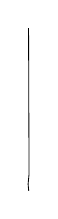
\begin{tikzpicture}[x=1mm,y=\baselineskip]
\draw[line width=0.3pt] (0,0) -- (0.06,-4.4) -- (-0.06,-4.7) -- (0.02,-4.9);
\end{tikzpicture}}
\uline{Proposition} For $\forall x\in\mathfrak X$, $\underline{O}_{\mathfrak X,x}$ is a valuation ring in $L$, with field of fractions $L$, and containing $K$. The map $x\longmapsto\underline{O}_{\mathfrak X,x}$ is a bijection from $\mathfrak X$ onto the set of these rings in $L$.
\margin{One could\newline start from an\newline excellent scheme\newline $X$, and construct\newline a relative $\mathfrak X$ over\newline it\unsure{\ldots|..}}

\uline{Proof} a) Let $f\in L\setminus\underline{O}_{\mathfrak X,x}$, we must prove $\frac1f\in\underline{O}_{\mathfrak X,x}$. Now $f=g/h$, \inserted{$g,h$}$\in\underline{O}_{X,a}$, where $X$ a \inserted{regular} model (proper), $a$ a point, $f,g$ \deleted{\unsure{prime} to each other} --- using resolution, \deleted{\unsure{one} \uline{\unsure{separates}} \unsure{the divisors}} \inserted{one may assume $\exists$ a regular system} of parameters, with $f,g$ monomials
\margin{121}
